\section{Il tensore}
Quando si lavora con gli algoritmi di machine learning, spesso occorre un modo per
rappresentare numericamente informazioni complessi come: suoni, immagini, testo o 
altre informazioni. 
In framework di machine learning e deep learning come TensorFlow e PyTorch,
la rappresentazione numerica delle informazioni è ottenuta attraverso
l'uso dei \textbf{Tensori}, che fungono da unità fondamentale 
per il calcolo sulla piattaforma. 

Un Tensore può essere definito come un oggetto matematico, una struttura dati 
multidimensionale che generalizza il concetto di scalare, vettore e 
matrice a $n$-dimensioni. Nel contesto della \textit{data science}, i tensori 
sono matrici multidimensionali di numeri che rappresentano dati complessi
\cite{Tensore_Fidacaro,Tensore_IBM,tensor_analytic,tensor_medium1,tensor_medium2,tensor_strano}. 

\subsection{Struttura e Caratteristiche dei Tensori}
Un tensore è definito da due proprietà principali che ne determinano la 
struttura \cite{Tensore_Fidacaro} :

\begin{itemize}
    \item \textbf{Rank (o dimensione)}:  
    Il rank di un tensore indica il numero di assi o direzioni lungo cui i dati 
    sono organizzati.
    
    \item \textbf{Shape (o forma)}:  
    La shape di un tensore è una tupla che specifica il numero di elementi lungo ogni asse. 
\end{itemize}

\subsection{Rappresentazione dei dati}
A seconda della loro dimensione (rank) e della forma (shape), i tensori possono modellare 
dati di diversa natura \cite{Tensore_Fidacaro}:

\begin{itemize}
    \item \textbf{Scalare}: Un tensore scalare rappresenta un singolo valore numerico. 
    Non ha direzioni o assi, ed è quindi di dimensione 0. 
    Ad esempio potrebbe essere il numero $5.5$ . 

    \item \textbf{Vettore}: Un vettore, ad esempio $[1\ 2\ 3]$, è una sequenza ordinata 
    di numeri disposti lungo un unico asse, e può essere rappresentato da un tensione di 
    dimensione 1.
  
    \item \textbf{Matrice}: una matrice come $\begin{bmatrix} 1 & 2 & 3 \\ 4 & 5 & 6 \end{bmatrix}$ 
    può essere vista come un tensore di dimensione 2.

    \item \textbf{Strutture 3D e oltre}: tutte le strutture matematiche con tre o più dimensioni, 
    ad esempio come 
    $\begin{bmatrix} 
    \begin{bmatrix} 1 & 2 \\ 3 & 4 \end{bmatrix} & 
    \begin{bmatrix} 5 & 6 \\ 7 & 8 \end{bmatrix} 
    \end{bmatrix}$, vengono rappresentati come tensori di dimensione 3 o superiore.
\end{itemize}

La figura (\ref{fig:Rappresentazione_Tensori}) mostra una rappresentazione grafica dei tensori al variare 
della dimensione

\begin{figure}[H]
    \centering
    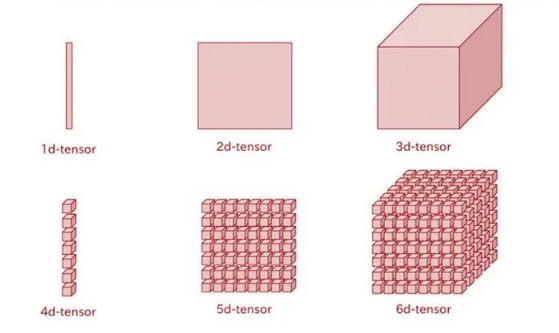
\includegraphics[width=0.72\textwidth]{Immagini/Generiche/esempio_tensori.png}
    \caption{Rappresentazione grafica dei tensori \cite{tensor_medium2} .}
    \label{fig:Rappresentazione_Tensori}
    %Figura 2.1: Esempio schematico di un neurone
\end{figure}


Ad esempio, se volessi utilizzare in python un tensore di pytorch per rappresentare 2 immagini 
RGB 3x3, il tensore apparirebbe così:
\begin{lstlisting}
images = torch.tensor([
    [
        [[255, 0, 0], [255, 255, 0], [0, 255, 0]], 
        [[0, 0, 255], [0, 255, 255], [0, 0, 255]], 
        [[255, 255, 255], [128, 128, 128], [0, 0, 0]]
    ], 
    [
        [[0, 0, 0], [128, 128, 128], [255, 255, 255]], 
        [[255, 0, 255], [255, 255, 0], [0, 255, 0]], 
        [[0, 0, 255], [255, 255, 255], [128, 128, 128]]
    ] 
])
\end{lstlisting}
Questo tensore così creato avrebbe shape $(2, 3, 3, 3)$ .


% \section{Operazioni tra tensori}
% Le operazioni sui tensori generalizzano quelle tra numeri, vettori e matrici. Tra le operazioni più comuni troviamo:

% \subsubsection{1. Somma tra tensori}
% Due tensori possono essere sommati solo se hanno la stessa forma (dimensioni). La somma viene eseguita elemento per elemento.

% \begin{itemize}
%     \item \textbf{Tensore A:} $\begin{bmatrix} 1 & 2 \\ 3 & 4 \end{bmatrix}$
%     \item \textbf{Tensore B:} $\begin{bmatrix} 5 & 6 \\ 7 & 8 \end{bmatrix}$
%     \item \textbf{Somma A + B:} $\begin{bmatrix} 1+5 & 2+6 \\ 3+7 & 4+8 \end{bmatrix} = \begin{bmatrix} 6 & 8 \\ 10 & 12 \end{bmatrix}$
% \end{itemize}

% \subsubsection{2. Moltiplicazione elemento per elemento (Hadamard product)}
% Due tensori con la stessa forma possono essere moltiplicati elemento per elemento.

% \begin{itemize}
%     \item \textbf{Tensore A:} $\begin{bmatrix} 1 & 2 \\ 3 & 4 \end{bmatrix}$
%     \item \textbf{Tensore B:} $\begin{bmatrix} 5 & 6 \\ 7 & 8 \end{bmatrix}$
%     \item \textbf{Prodotto Hadamard AB:} $\begin{bmatrix} 1 \cdot 5 & 2 \cdot 6 \\ 3 \cdot 7 & 4 \cdot 8 \end{bmatrix} = \begin{bmatrix} 5 & 12 \\ 21 & 32 \end{bmatrix}$
% \end{itemize}

% \subsubsection{3. Prodotto scalare (dot product)}
% Il prodotto scalare tra due tensori è possibile quando una delle dimensioni del primo tensore corrisponde a una delle dimensioni del secondo.

% \begin{itemize}
%     \item \textbf{Tensore A (2x3):} $\begin{bmatrix} 1 & 2 & 3 \\ 4 & 5 & 6 \end{bmatrix}$
%     \item \textbf{Tensore B (3x2):} $\begin{bmatrix} 7 & 8 \\ 9 & 10 \\ 11 & 12 \end{bmatrix}$
%     \item \textbf{Prodotto A · B:} 
%     $\begin{bmatrix} 
%     (1 \cdot 7 + 2 \cdot 9 + 3 \cdot 11) & (1 \cdot 8 + 2 \cdot 10 + 3 \cdot 12) \\ 
%     (4 \cdot 7 + 5 \cdot 9 + 6 \cdot 11) & (4 \cdot 8 + 5 \cdot 10 + 6 \cdot 12) 
%     \end{bmatrix} = \begin{bmatrix} 58 & 64 \\ 139 & 154 \end{bmatrix}$
% \end{itemize}

% \subsubsection{4. Prodotto tensore (tensor product)}
% Il prodotto tensore tra due tensori crea un tensore di ordine più alto.

% \begin{itemize}
%     \item \textbf{Tensore A:} $[1, 2]$
%     \item \textbf{Tensore B:} $[3, 4]$
%     \item \textbf{Prodotto AB:} $\begin{bmatrix} 1 \cdot 3 & 1 \cdot 4 \\ 2 \cdot 3 & 2 \cdot 4 \end{bmatrix} = \begin{bmatrix} 3 & 4 \\ 6 & 8 \end{bmatrix}$
% \end{itemize}

% \subsubsection{5. Trasposizione}
% La trasposizione di un tensore consiste nello scambiare l'ordine di alcune delle sue dimensioni. Per esempio, in una matrice, si scambiano righe e colonne.

% \begin{itemize}
%     \item \textbf{Tensore A:} $\begin{bmatrix} 1 & 2 & 3 \\ 4 & 5 & 6 \end{bmatrix}$
%     \item \textbf{Trasposta $A^T$:} $\begin{bmatrix} 1 & 4 \\ 2 & 5 \\ 3 & 6 \end{bmatrix}$
% \end{itemize}

% \subsubsection{6. Riduzione di dimensioni}
% I tensori possono essere ridotti lungo una determinata dimensione, sommando o calcolando la media degli elementi.

% \begin{itemize}
%     \item \textbf{Tensore A (2x3):} $\begin{bmatrix} 1 & 2 & 3 \\ 4 & 5 & 6 \end{bmatrix}$
%     \item \textbf{Somma lungo la prima dimensione:} $[1+4, 2+5, 3+6] = [5, 7, 9]$
%     \item \textbf{Somma lungo la seconda dimensione:} $[1+2+3, 4+5+6] = [6, 15]$
% \end{itemize}

\subsection{I tensori nelle reti neurali}
Come si vedrà più avanti, il funzionamento delle reti neurali si basa 
su delle operazioni matematiche lineari, come ad esempio il prodotto matriciale. 
I tensori funzionano in modo simile ai \textit{ndarray} usati in NumPy, ma a 
differenza dei \textit{ndarray}, che possono essere eseguiti solo su unità 
di elaborazione centrali (CPU), i tensori possono essere eseguiti anche
su appositi acceleratori hardware, come le unità di elaborazione grafica (GPU) e 
unità di elaborazione per Tensori (TPU) .
Le GPU e TPU consentono un calcolo notevolmente più veloce rispetto alle CPU, 
il che rappresenta un grande vantaggio dati gli enormi volumi di dati e 
l'elaborazione parallela tipici del deep learning.
Riassumendo, utilizzare i tensori per rappresentare le informazioni e 
svolgere calcoli, permette di sfruttare l'accelerazione hardware 
offerta da GPU e TPU per parallelizzare le operazioni matematiche e 
svolgerle in modo efficiente.
I tensori, oltre ad essere utilizzati per codificare gli input e gli output 
di un modello di una rete neurale, vengono utilizzati anche per 
codificare i parametri del modello: pesi, pregiudizi e gradienti che 
vengono "appresi". 
Questa proprietà dei tensori consente la differenziazione automatica 
(calcolo automatico delle derivate), una delle funzioni più importanti 
di PyTorch \cite{Tensore_Fidacaro,Tensore_IBM,tensor_analytic,tensor_medium1,tensor_medium2,tensor_strano}.

\subsection{Velocità computazionale dei tensori}
Per dare idea dei vantaggi computazionali dell'utilizzo dei tensori, 
realizziamo un test in cui confrontiamo le prestazioni degli array \textit{NumPy}
e dei tensori di \textit{PyTorch} nella moltiplicazione tra matrici.
In questo test inizializziamo casualmente  due \textit{arrays/tensors} 4D
e misureremo il tempo necessario a svolgere la moltiplicazione tra i due.
Come dispositivo di accelerazione hardware utilizzeremo una GPU, la cui 
selezione avviene tramite il comando \texttt{torch.device("cuda")}.
Qualora si volesse selezionare una specifica GPU, è possibile aggiungere un numero dopo 
\texttt{"cuda"} il numero della GPU (ad esempio \texttt{"cuda:1"} per selezionare la 
seconda GPU). Se il numero viene omesso, il comando utilizzerà automaticamente 
la GPU \texttt{"cuda:0"}. Il codice del test è il seguente:

\begin{lstlisting}
import torch
import numpy as np
import time

dim_max = 110
shapes = []
device = torch.device("cuda")

for dim in range(5, dim_max + 1, 5):
    shapes.append((dim, dim, dim, dim))

for shape in shapes:
    array1 = np.random.rand(*shape)
    array2 = np.random.rand(*shape)
    tensor1 = torch.rand(*shape).to(device)
    tensor2 = torch.rand(*shape).to(device)

    start_time = time.perf_counter()
    np.matmul(array1, array2)
    dt = time.perf_counter() - start_time
    cpu_times.append(dt)

    torch.cuda.synchronize() 
    start_time = time.perf_counter()
    torch.matmul(tensor1, tensor2)
    torch.cuda.synchronize()
    gpu_times.append(time.perf_counter() - start_time)
plot(shapes, cpu_times, gpu_times)

\end{lstlisting}

Eseguito il test di confronto, questi sono i risultati che otteniamo: 

\begin{figure}[H]
    \centering
    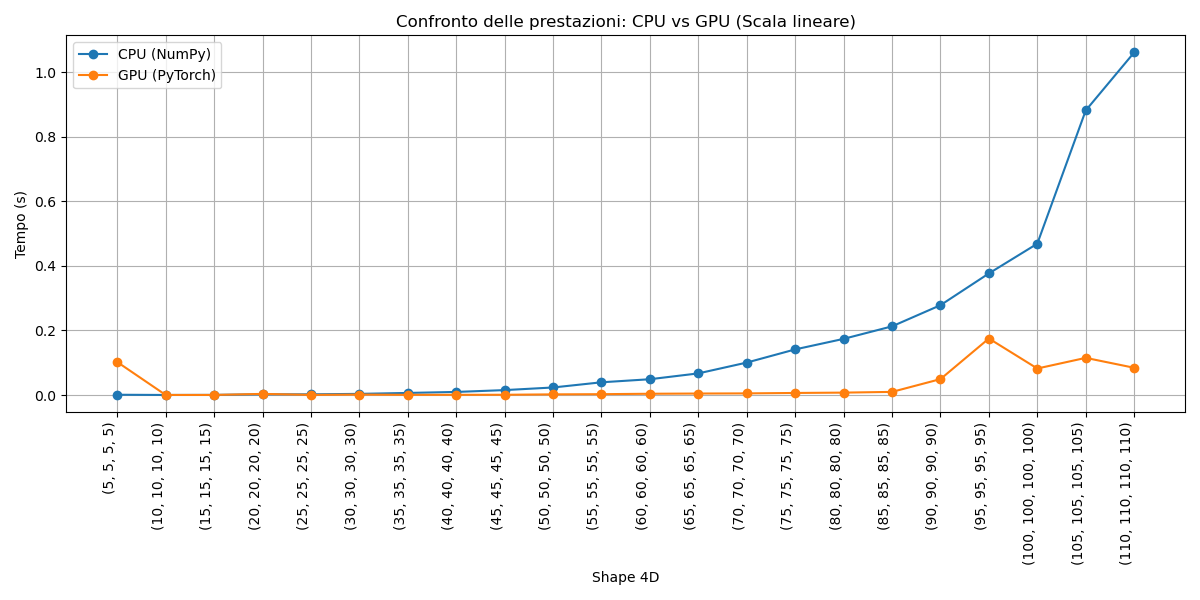
\includegraphics[width=0.92\textwidth]{Immagini/Grafici/Tensor_lin_plot.png}
    \caption{Grafico lineare del paragone array-tensore }
\end{figure}

\begin{figure}[H]
    \centering
    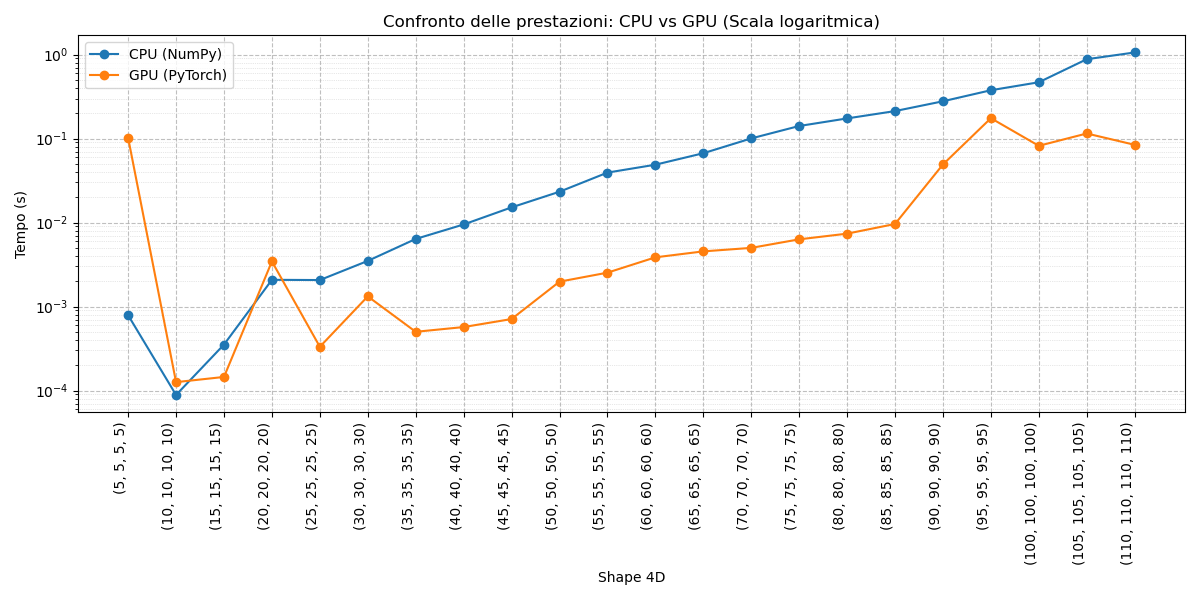
\includegraphics[width=0.92\textwidth]{Immagini/Grafici/Tensor_log_plot.png}
    \caption{Grafico logaritmico del paragone array-tensore }
\end{figure}
 

Come possiamo osservare, per dimensioni ridotte, i calcoli eseguiti con gli array
di \textit{NumPy} risultano essere molto più veloci rispetto a quelli svolti 
con i tensori di \textit{PyTorch}.
Ma all'aumentare delle dimensioni, i calcoli eseguiti su GPU 
risultano essere da 24 a 52 volte più veloci rispetto a quelli su CPU.
Le prestazioni possono dipendere sia dall'implementazione del codice, sia 
dall'hardware utilizzato. Ma questa velocità di elaborazione offerta dalle GPU è uno 
dei motivi principali per cui i tensori (e non gli array) sono 
ampiamente utilizzati nel deep learning per rappresentare i dati ed eseguire operazioni 
matematiche.

